\documentclass[border=10pt]{standalone}
\usepackage[svgnames]{xcolor}
\usepackage{amsmath}
\usepackage{pgfplots}
\pgfplotsset{compat=newest}
\usepackage[sfdefault]{FiraSans}
\usepackage{FiraMono}
\renewcommand*\familydefault{\sfdefault}
\begin{document}
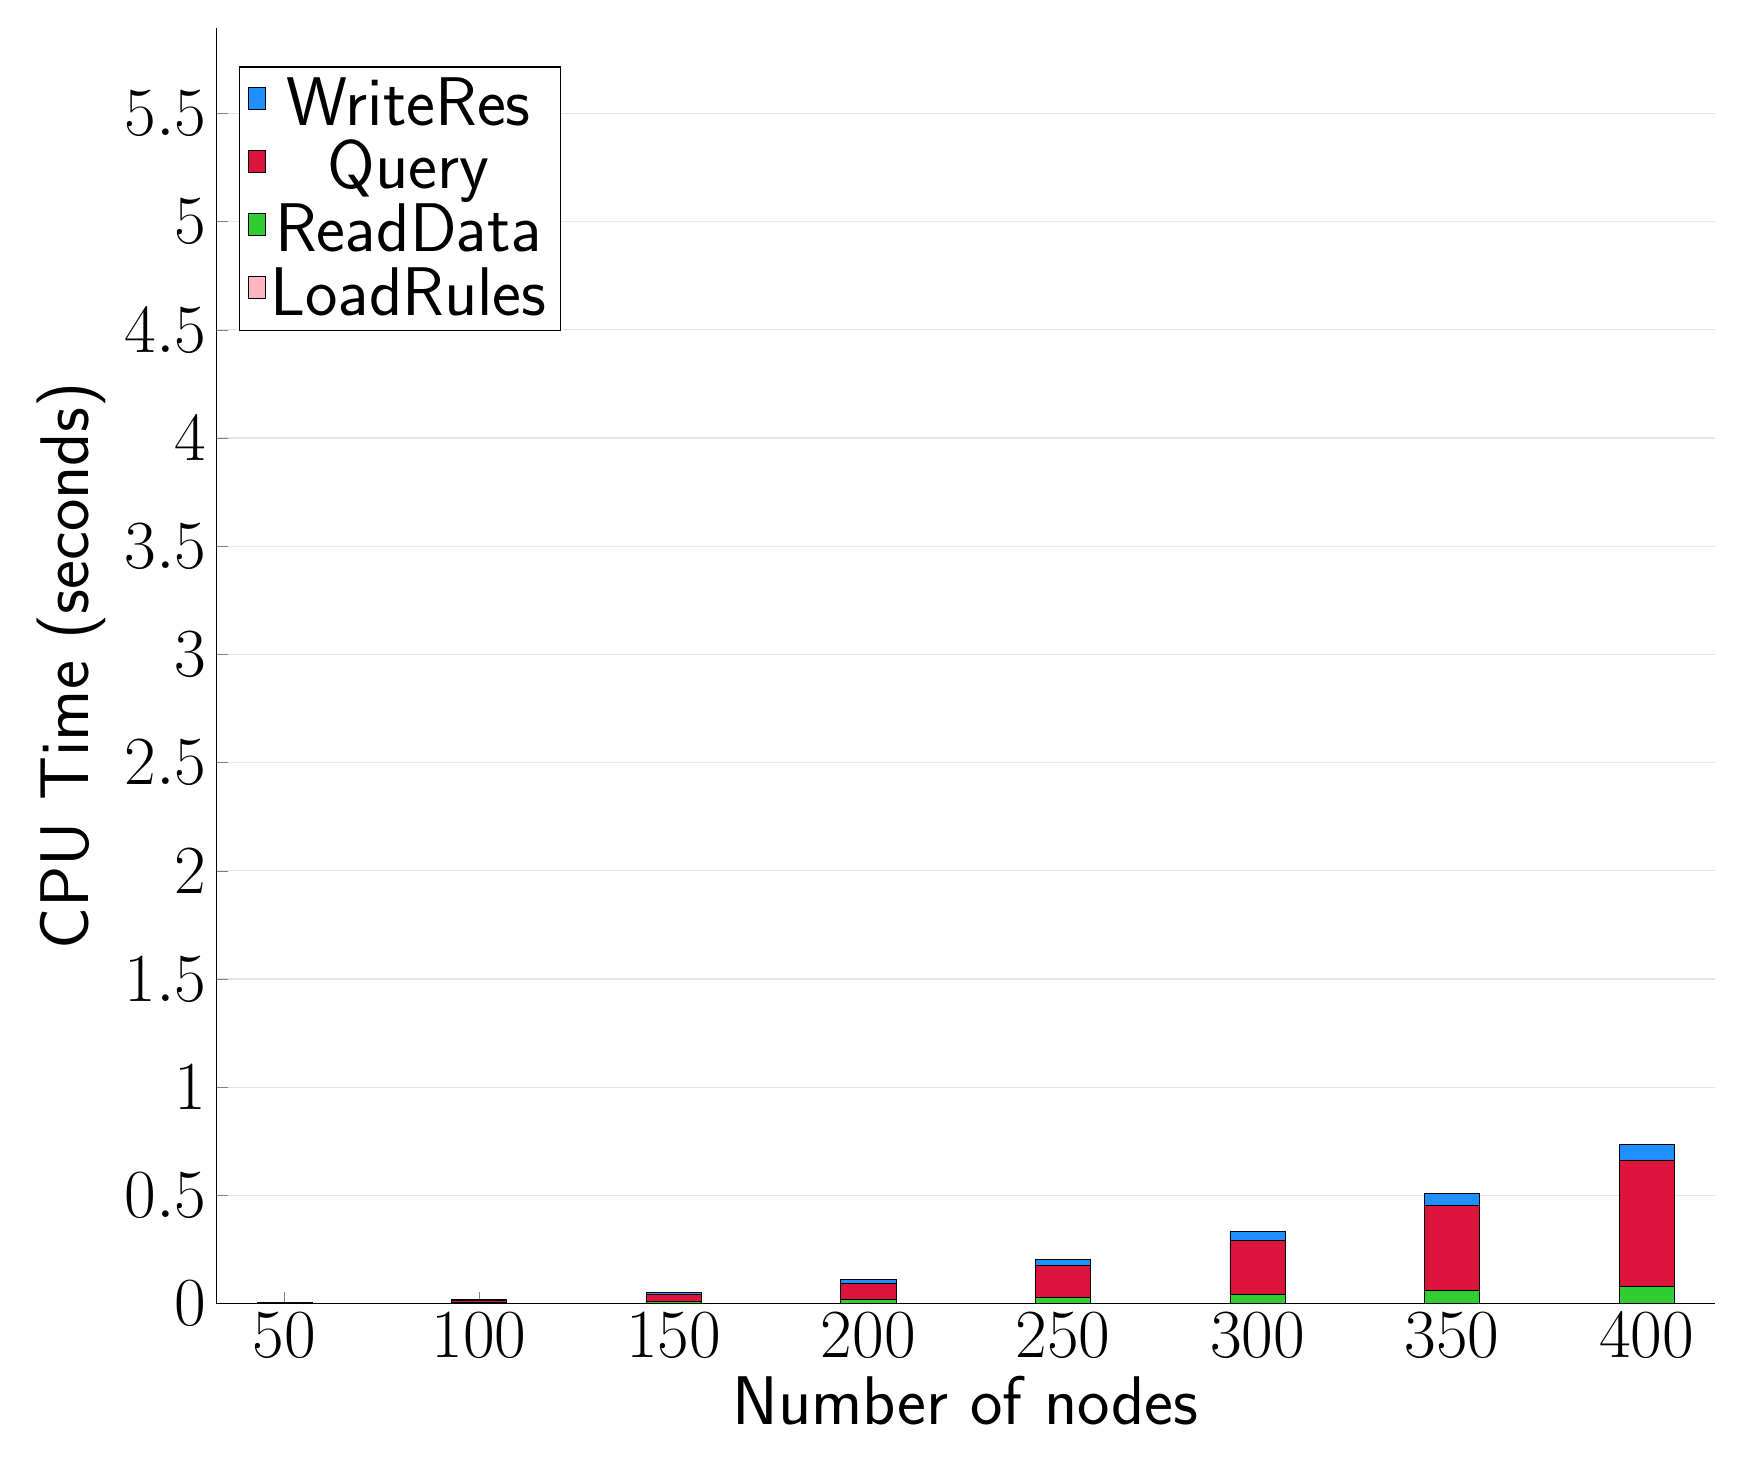
\begin{tikzpicture}
	\begin{axis}[
			ybar stacked,
			width=1.7\textwidth,
			bar width=0.7cm,
			ymajorgrids, tick align=inside,
			major grid style={draw=gray!20},
			xtick=data,
			ymin=0, ymax=5.893940000000001,
			axis x line*=bottom,
			axis y line*=left,
			enlarge x limits=0.05,
			legend style={
					at={(0.23, 0.97)},
					anchor=north east,
					legend columns=1,
					font=\Huge,
				},
			ylabel={CPU Time (seconds)},
			xlabel={Number of nodes},
			label style={font=\Huge},
			tick label style={font=\Huge},
		]
		\addlegendimage{fill=DodgerBlue, draw=black, line width=0.2pt}
		\addlegendentry{WriteRes}
		\addlegendimage{fill=Crimson, draw=black, line width=0.2pt}
		\addlegendentry{Query}
		\addlegendimage{fill=LimeGreen, draw=black, line width=0.2pt}
		\addlegendentry{ReadData}
		\addlegendimage{fill=LightPink, draw=black, line width=0.2pt}
		\addlegendentry{LoadRules}
		\addplot +[fill=LightPink, draw=black, line width=0.2pt] coordinates {
				(50, 0.0006057000000000001)
				(100, 0.0006084000000000003)
				(150, 0.0006120999999999998)
				(200, 0.0006119999999999999)
				(250, 0.0006014999999999998)
				(300, 0.0006125)
				(350, 0.0006228999999999998)
				(400, 0.0006317)
			};
		\addplot +[fill=LimeGreen, draw=black, line width=0.2pt] coordinates {
				(50, 0.0011666)
				(100, 0.0044178)
				(150, 0.010223)
				(200, 0.018557599999999997)
				(250, 0.029586499999999998)
				(300, 0.0433033)
				(350, 0.060255899999999994)
				(400, 0.079759)
			};
		\addplot +[fill=Crimson, draw=black, line width=0.2pt] coordinates {
				(50, 0.0013027)
				(100, 0.0095498)
				(150, 0.0315914)
				(200, 0.0746347)
				(250, 0.1458401)
				(300, 0.24822100000000002)
				(350, 0.3940025)
				(400, 0.5842841999999999)
			};
		\addplot +[fill=DodgerBlue, draw=black, line width=0.2pt] coordinates {
				(50, 0.0011030999999999999)
				(100, 0.0046101)
				(150, 0.010584199999999998)
				(200, 0.0177863)
				(250, 0.0273495)
				(300, 0.04059600000000001)
				(350, 0.05494140000000001)
				(400, 0.07059300000000002)
			};
	\end{axis}
\end{tikzpicture}

\end{document}
